\setchapterimage{Fond_ALG.png}
\setchapterpreamble[u]{\margintoc}
\chapter{Initiation à l'algorithmique et à la programmation}

\marginnote[4cm]{
\begin{itemize} 
\item Choisir un type de variable.
\item Concevoir un algorithme utilisant une structure conditionnelle (Si), une structure itérative (while), une structure itérative (for).
\item Concevoir une fonction.
\item Manipuler des listes.
\item Instruction et expression.
\end{itemize}
}
\begin{center}
En cas de besoin, je rappelle ici le site de la classe en informatique : 

\url{https://ptsilamartin.github.io/}
\end{center}


\section{Avant-Propos}
\subsection{Définitions}

\begin{defi}[Informatique -- Wikipedia]
L'informatique est un domaine d'activité scientifique, technique, et industriel concernant le traitement automatique de l'information numérique par l'exécution de programmes informatiques hébergés par des dispositifs électriques-électroniques : des systèmes embarqués, des ordinateurs, des robots, des automates, etc.
\end{defi}

\begin{defi}[Algorithmique -- Wikipedia]
Un algorithme est une méthode générale pour résoudre un type de problèmes. Il est dit correct lorsque, pour chaque instance du problème, il se termine en produisant la bonne sortie, c'est-à-dire qu'il résout le problème posé.
\end{defi}

L'efficacité d'un algorithme est mesurée notamment par :
\begin{itemize}
\item sa durée de calcul ;
\item sa consommation de mémoire vive (en partant du principe que chaque instruction a un temps d'exécution constant) ;
\item la précision des résultats obtenus (par exemple avec l'utilisation de méthodes probabilistes) ;
\item sa scalabilité (son aptitude à être efficacement parallélisé) ;
\item etc.
\end{itemize}

Les ordinateurs sur lesquels s'exécutent ces algorithmes ne sont pas infiniment rapides, car le temps de machine reste une ressource limitée, malgré une augmentation constante des performances des ordinateurs. Un algorithme sera donc dit performant s'il utilise avec parcimonie les ressources dont il dispose, c'est-à-dire le temps CPU, la mémoire vive et (aspect objet de recherches récentes) la consommation électrique. L’analyse de la complexité algorithmique permet de prédire l'évolution en temps calcul nécessaire pour amener un algorithme à son terme, en fonction de la quantité de données à traiter.

\begin{defi}[Programmation -- Wikipedia]
La programmation, appelée aussi codage dans le domaine informatique, désigne l'ensemble des activités qui permettent l'écriture des programmes informatiques. C'est une étape importante du développement de logiciels.

L'écriture d'un programme se fait dans un langage de programmation. Un logiciel est un ensemble de programmes (qui peuvent être écrits dans des langages de programmation différents) dédié à la réalisation de certaines tâches par un (ou plusieurs) utilisateurs du logiciel.

\end{defi}

La programmation représente donc ici la rédaction du code source d'un logiciel. On utilise plutôt le terme développement pour dénoter l'ensemble des activités liées à la création d'un logiciel et des programmes qui le composent. Cela inclut la spécification du logiciel, sa conception, puis son implémentation proprement dite au sens de l'écriture des programmes dans un langage de programmation bien défini, ainsi que la vérification de sa correction, etc.

\subsection{Environnement de développement}
Pour répondre à un problème informatique, on pourra réfléchir à l'algorithme permettant de le résoudre. Une des premières approches consiste donc à utiliser un papier et un crayon pour proposer une réponse structurée au problème.

Il faudra ensuite traduire cet algorithme dans un langage de programmation. Nous utiliserons pour cela \lstinline{Python}.

Pour programmer en \lstinline{Python} il est nécessaire d'utiliser un éditeur de texte (pour écrire le code) et un interpréteur pour exécuter le code. 
En règle générale, on utilise pour cela un environnement de développement (IDE). On pourra \textbf{Pyzo} ou \textbf{Spyder} (ou tout autre environnement vous paraissant satisfaisant). 

\begin{figure}[H]
\centering
%\begin{center}
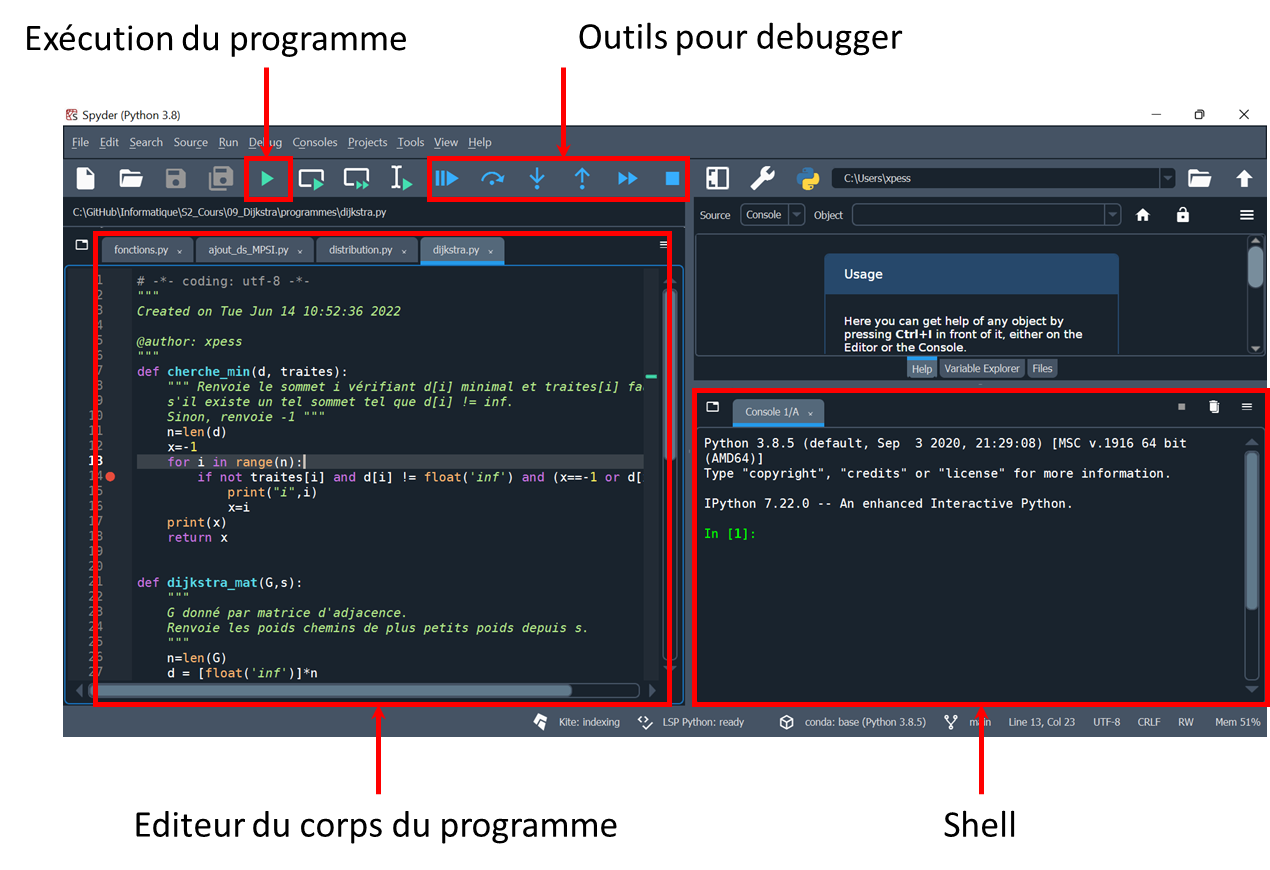
\includegraphics[width=12cm]{Spyder.png}
%\end{center}
\end{figure}

\section{Variables, Types}

\subsection{Quelques définitions}
\begin{defi}[Valeurs]
Les valeurs désignent les données manipulées par un algorithme ou une fonction. Une valeur 
peut ainsi être  : un nombre, un caractère, une chaîne de caractères, une valeur de vérité 
(\lstinline{Vrai} ou \lstinline{Faux}) \textit{etc}.

En Python, comme dans la plupart des langages de programmation, ces valeurs sont \textbf{typées} selon l'objet qu'elles représentent : il y a ainsi des valeurs de \textbf{type} entier, flottant, chaîne de caractères, booléens ...   Leur représentation en mémoire varie beaucoup d'un langage à l'autre, mais ce sont souvent les mêmes objets que l'on 
cherche à traduire.
\end{defi}

\begin{defi}[Expression]
Une expression est une suite de caractères faisant intervenir des valeurs et des 
opérations, afin d'obtenir une nouvelle valeur. Pour calculer cette nouvelle valeur,
la machine doit {évaluer} l'expression. Voici des exemples d'expressions : \lstinline{42}, \lstinline{1+4}, 
\lstinline{1.2 / 3.0}, \lstinline{x+3}.
\end{defi}

En Python, pour évaluer une expression, il suffit de la saisir dans un interpréteur (console, shell), qui
calcule et affiche alors la valeur qu'il a calculée.
\begin{lstlisting}
>>> 42
	42
>>> 1+4
	5
\end{lstlisting}


\begin{defi}[Variable]
Une \textbf{variable} désigne une zone mémoire de l'ordinateur dans la RAM.
Il s'agit d'un endroit où l'on peut \textbf{stocker} une valeur, y \textbf{accéder} et 
\textbf{changer} cette valeur.
\end{defi}

Pour faire référence à une variable, on utilise un nom de variable, en général composé d'une ou 
plusieurs lettres. Dans la mesure du possible, on choisit un nom explicite, ce qui permet une 
meilleure lecture du programme.



\begin{defi}[Affectation]
Quand on stocke une valeur \lstinline{d} dans une variable \lstinline{var}, on dit que l'on 
\textbf{affecte} \lstinline{d} à la variable \lstinline{var}. La valeur
\lstinline{d} est encore appelée \textbf{la donnée}.
\end{defi}

En Python , cette affectation est faite avec la commande \lstinline{=}, comme suit.  

\begin{lstlisting}
>>> var  = 1
\end{lstlisting}





\subsection{Types simples}

En programmation, associer un type à une valeur permet :
\begin{itemize}
\item de classer les valeurs en catégories similaires. Par exemple, tous les
entiers (type int), tous les flottants (type float)...
\item de contrôler quelles opérations sont faisables sur ces valeurs : par
exemple, tout entier (type int) pourra être utilisé dans une soustraction, ..., alors 
qu'une chaîne ne le pourra pas. Il sera également impossible d'additioner un entier et un booléen. 
                                     
\end{itemize}

Une expression n'a a priori pas de type, car le type de la valeur qu'elle renvoie dépend des types 
des sous-expressions. Ainsi \lstinline{a+b} sera un entier (resp. un flottant, une chaîne) si 
\lstinline{a} et \lstinline{b} le sont, mais sera un flottant si \lstinline{a} est un entier et \lstinline{b} 
un flottant.


%\begin{xxpyconsole}%~\\ \vspace{-.5cm}
Pour afficher le type d'une valeur ou d'une expression après l'avoir évaluée, on utilise 
\lstinline{type}. 
\begin{lstlisting}
>>> type(42)
	int
>>> type(1.2/3.0)
	float
\end{lstlisting}
%Le mot qui suit \lstinline{class} indique le type de la valeur, entier (\lstinline{int} en anglais) pour 
%la première et flottant (\lstinline{float} en anglais) pour la seconde. Le mot \lstinline{class} fait 
%référence au fait que Python, est un langage {orienté objet}, ce que nous ignorerons pour 
%l'instant.\\
%\end{xxpyconsole}





%\subsubsection{Entiers}
\marginnote[4cm]{Il est possible de faire une division entre deux nombre entiers en utilsant le symbole \lstinline{/}, mais le résultat ne sera pas un nombre de type \lstinline{int} mais de type \lstinline{float}.}
\begin{defi}[Entiers]
Ce type est noté \lstinline{int} en Python .\\
\begin{itemize}
\item \textbf{Constantes :} ce sont les entiers relatifs écrits en base 10. Ils ne sont pas 
bornés en Python .
\item \textbf{Opérateurs :}
\begin{enumerate}
 \item $+$ : addition usuelle;
 \item $-$ : soustraction usuelle (\lstinline{15-9} renvoie \lstinline{6}), mais aussi opposé (\lstinline{-4});
\item  $//$ : {division entière} : \lstinline{a//b} correspond au quotient de la 
division euclidienne de \lstinline{a} par \textbf{b} si \lstinline{b} est strictement positif 
(\lstinline{256 // 3} renvoie \lstinline{85} car $256 = 85*3 + 1$). Mais si \lstinline{b} est strictement 
négatif, alors \lstinline{a//b} renvoie ce quotient moins 1 ($15 = (-4)\times(-4)-1=(-4)\times(-3)+3$, 
le quotient de la division euclidienne de 15 par $-4$ est $-3$, mais \lstinline{15//-4} renvoie 
\lstinline{-4}). Cette division n'est pas définie si \lstinline{b} est nul;
\item $\%$ : {modulo} : même remarque que dans le point précédent, relativement au reste de la 
division euclidienne cette fois (\lstinline{256 \% 3} renvoie 
\lstinline{1}, \lstinline{15\%-4} renvoie \lstinline{-1}).
\item $**$ : exponentiation (\lstinline{2**3} renvoie \lstinline{8}).
\end{enumerate}
\end{itemize}
Les {règles de précédence}, autrement dit les règles de priorité entre opérations, sont 
similaires aux règles mathématiques usuelles.
\end{defi}
%\subsubsection{Flottants}
\begin{defi}[Flottants]
Ce type est noté \lstinline{float} en Python .
\begin{itemize}
\item  \textbf{Constantes :} ce sont les {nombres à virgule flottante}. Nous en
donnerons une définition précise dans un chapitre ultérieur : pour simplifier, disons pour 
l'instant que ce sont des nombres à virgule, avec un nombre borné de chiffres dans leur écriture.
\item \textbf{Opérateurs : }
\begin{enumerate}
 \item $+$ : addition usuelle;
 \item $-$ : soustraction usuelle, et aussi opposé;
\item  $/$ : division usuelle;
\item $**$ : exponentiation. %Remarquer la différence entre \lstinline{2\raisebox{0.3ex}{**}100} et  \lstinline{2.\raisebox{0.3ex}{**}100} ou \lstinline{2\raisebox{0.3ex}{**}100.}.
\end{enumerate}
\end{itemize}
%\noindent\textbf{Avertissement :} ce qui précédé est valable en Python 3. Attention à l'opérateur 
%\lstinline{/} en Python 2 !!!!
\end{defi}

%\subsubsection{Booléens}


\begin{defi}[Expression -- Booléen]
%\footnote{Le mot {booléen} a été donné en hommage au mathématicien  britannique George Boole.} }}
Ce type est noté \lstinline{bool} en Python.
\begin{itemize}
\item \textbf{Constantes :} il y en a deux : \lstinline{True} et \lstinline{False}.
\item \textbf{Opérateurs :}
\begin{enumerate}
 \item \lstinline{not} : négation usuelle;
 \item \lstinline{and} : conjonction usuelle;
 \item \lstinline{or} : disjonction usuelle.
\end{enumerate}
\item \textbf{Opérateurs de comparaison :}
\begin{enumerate}
 \item \lstinline{==} : test d'égalité : \lstinline{2==3} renvoie \lstinline{False}, \lstinline{4==4} renvoie 
\lstinline{True}; %Problème : \lstinline{0.1+0.2==0.3} renvoie \lstinline{False} ! Nous y reviendrons plus tard. Il ne faut pas confondre \lstinline{==} avec \lstinline{=}, symbole de l'{affectation}.
 \item \lstinline{!=} : \lstinline{a != b} est une écriture équivalente à \lstinline{not (a == b)};
 \item \lstinline{<,>,<=,>=} : ce à quoi on s'attend.
\end{enumerate}
\end{itemize}
\end{defi}


\begin{exemple}
\lstinline{True or False} renvoie \lstinline{True}. 

\lstinline{not(False or True) and True} renvoie \lstinline{False}.
\end{exemple}

\begin{remarque}
Python \ permet les chaînes de comparaisons : \lstinline{1<2<3} renvoie
\lstinline{True}, et \lstinline{(1<2<-2) and (-5<2<6)} renvoie \lstinline{False}.
\end{remarque}

\subsection{Conversions \textit{-- Cast}}

Il est possible de convertir en entier en flottant avec la fonction \lstinline{float}. La réciproque est possible dans une certaine 
mesure : \lstinline{float(2)} renvoie \lstinline{2.0}, \lstinline{int(2.0)} renvoie \lstinline{2}, mais \lstinline{int(2.6)} renvoie \lstinline{2} et 
\lstinline{int(-3.6)} renvoie \lstinline{-3}.

La fonction \lstinline{int} appliquée à un nombre flottant procède donc à une troncature, ce n'est pas la fonction donnant la partie entière d'un nombre flottant (fonction \lstinline{floor} du module \lstinline{math}).
%
%\subsection{Types composés}
%\begin{defi}
%On dit qu'une valeur est de type composé si elle est formée à partir de plusieurs autres 
%valeurs de types plus simples. De nombreuses constructions sont définies sur tous les types 
%composés.
%\end{defi}
%
%\subsubsection{$n$-uplets ou tuples}
%
%\begin{defi}[Tuple]
%Ce type est noté \lstinline{tuple} en Python .
%\begin{itemize}
%\item \textbf{Construction et composantes :} les $n$-uplets généralisent les couples. Un couple s'écrira \lstinline{(a,b)}, un triplet 
%\lstinline{(a,b,c)} ... etc. Il existe même des 1-uplets : il faut les écrire \lstinline{(a,)}.\\%, et non  \lstinline{(a)} : cette dernière écriture est équivalente à \lstinline{a}, tout simplement.\\
%Il n'est pas obligatoire que les éléments d'un tuple soient de même type. Par exemple, 
%\lstinline{(1,1.2,True)} est un triplet tout à fait valable.\\
%On accède à la $k\ieme$ coordonnée d'un tuple \lstinline{t} par la commande \lstinline{t[k]}. Attention : 
%\textbf{en Python , les coordonnées sont numérotées à partir de 0} ! On dit que $k$ est 
%l'{indice} de \lstinline{t[k]}. Ainsi, si \lstinline{t = (1,2,3)}, \lstinline{t[0]} vaut 1, 
%\lstinline{t[2]} vaut 3, et \lstinline{t[3]} n'existe pas.\\
%On dit que les tuples sont \textbf{immuables} ou \textbf{non mutables}: il n'est pas possible de changer un élément d'un 
%tuple.
%\item \textbf{Opérateurs :}
%\begin{enumerate}
% \item $+$ : concaténation. \lstinline{(1,2,3)+(1,4,5,6)} renvoie \lstinline{(1,2,3,1,4,5,6)};
% \item \lstinline{len} : {longueur} du tuple. \lstinline{len(1,2,3)} renvoie \lstinline{3};
% \item \lstinline{in} : test d'appartenance. \lstinline{3 in (1,2,3)} renvoie \lstinline{True}, alors que 
%\lstinline{3 in (1,2,4,5)} renvoie \lstinline{False};
%\item le {slicing}, qui permet de construire des sous-tuples : \lstinline{(5,2,6,7,8,9)[1:5]} 
%renvoie \lstinline{(2,6,7,8)} (attention à la borne de droite !).\\
%\end{enumerate}
%\end{itemize}
%\end{defi}
%
%\subsubsection{Chaînes de caractères}
%\begin{defi}[Chaînes de caractères]
%Ce type est noté \lstinline{str} en Python , pour {string} en anglais.
%\begin{itemize}
%\item \textbf{Construction et composantes :} ce sont des suites finies de caractères, un caractère étant en python un caractère du clavier. On 
%les note entre guillemets ou apostrophes : \lstinline{``Ceci est une chaîne de caractères''} ou  
%\lstinline{'Ceci est une chaîne de caractères'}. La chaîne vide se note \lstinline{``}\lstinline{''} ou 
%\lstinline{''}. Un caractère est une chaîne de longueur 1.\\
%On accède aux composantes d'une chaîne de la même manière que pour un tuple.
%\item \textbf{Opérateurs :} ce sont les mêmes que pour les tuples.
%\end{itemize}
%\end{defi}
%
%\subsection{Listes}
%\marginnote{
%$>>>$\lstinline{ L = [1,2,3] } \\
%$>>>$\lstinline{ L[0] = 4 } \\
%$>>>$\lstinline{ L } \\
%$\quad $ \lstinline{[4,2,3]}
%%\end{lstlisting}
%}
%
%\begin{defi}[Listes]
%Ce type est noté \lstinline{list} en Python .
%
%Comme les tuples, les {listes} sont des suites finies de valeurs arbitraires, mais cette fois 
%ils sont \textbf{mutables} : on peut changer la valeur d'une composante d'une liste.\\
%Les listes s'écrivent entre crochets. On change la valeur de la $k\ieme$ composante d'une liste 
%\lstinline{L} grâce à la commande \lstinline{L[k] = n}, où \lstinline{n} est la nouvelle valeur.
%
%Les autres opérateurs sont les mêmes que pour les tuples et les chaînes. Nous reviendrons plus tard sur les listes.
%\end{defi}

%\subsection{Conversions}
%
%On peut convertir des types simples en chaînes avec la fonction \lstinline{str} : \lstinline{str(2.3)} 
%renvoie \lstinline{'2.3'}.\\
%À l'inverse, \lstinline{int, float} et \lstinline{bool} permettent de faire l'inverse quand cela est 
%cohérent : \textbf{bool('True')} renvoie \lstinline{True}, mais \lstinline{int('2.3')} renvoie une 
%erreur.\\
%
%Il est également possible de passer d'un type composé à un autre grâce aux fonctions \lstinline{str}, 
%\lstinline{tuple} et \lstinline{list} : \lstinline{str((1,'a',[1,2]))} renvoie \lstinline{''(1,'a',[1,2])''}, 
%\lstinline{tuple([1,2,3] )} renvoie \lstinline{(1,2,3)} et \lstinline{list('Coucou ?')} renvoie 
%\lstinline{['C', 'o', 'u', 'c', 'o', 'u', ' ', '?']}.

\subsection{Affectation}

\begin{defi}[Affectation]
Quand on stocke une valeur \lstinline{d} dans une variable \lstinline{var}, on dit que l'on 
\textbf{affecte} \lstinline{d} à la variable \lstinline{var}. La valeur
\lstinline{d} est encore appelée \textbf{la donnée}.
\end{defi}

En Python , cette affectation est faite avec la commande \lstinline{=}, comme suit.  

\begin{lstlisting}
>>> var  = 1
\end{lstlisting}


Les variables (et donc l'affectation) sont incontournables : si vous ne stockez pas une donnée 
(résultat par exemple d'un calcul), vous ne pourrez pas la réutiliser, ni la modifier.

%\begin{xxpyconsole}~\\ \vspace{-.5cm}%\begin{exemple}~
\begin{lstlisting}
>>> x = 42                    # x prend la valeur 42.
>>> x = x + 2                 # On additionne à la donnée stockée dans x 
                              # le nombre 2 et on stocke le résultat  
                              # de nouveau dans x.
>>> x                    # on accède à la valeur qui est mémorisée dans x.
	44
\end{lstlisting}
%\end{xxpyconsole}
%\end{exemple}

Dans la variable affectée, la nouvelle donnée \og écrase\fg\ la donnée précédente : on perd son 
ancienne valeur.

Dans un programme Python, on utilisera l'instruction \lstinline{print(x)}
pour afficher dans la console la valeur de la variable \lstinline{x}.

Il est également possible d'affecter des valeurs à plusieurs variables en une fois, en utilisant 
des tuples. Ainsi : \lstinline{a,b = (1,2)} affecte la valeur 1 à \lstinline{a} et la valeur 2 à 
\lstinline{b}.


\begin{remarque}
En Python, le \textbf{typage} des variables est \textbf{dynamique}. Cela signifie que lorsqu'on affecte une valeur à une variable, Python reconnaît automatiquement le type de la valeur. Ce n'est pas le cas de tous les langages de programmation.
%Par exemple, le \lstinline{C} n'est pas typé dynamiquement. Il faut alors déclarer une variable avec un type, puis affecter la valeur. 
\end{remarque}


\begin{remarque}[ -- Affectation multiple]
En Python, il est possible d'affecter plusieurs variables à la fois.

\begin{lstlisting}
>>> a,b,c = 1,2,3
\end{lstlisting}

est équivalent à 


\begin{lstlisting}
>>> a = 1
>>> b = 2
>>> c = 3
\end{lstlisting}
\end{remarque}

\subsubsection*{Affichage d'une variable}
Pour afficher une variable, on peut la saisir dans le shell ou utiliser la fonction \lstinline{print}.
\begin{lstlisting}
>>> a = 1
>>> print(a)
1
\end{lstlisting}


\subsubsection*{Notion d'adressage}

En Python, le passage des variables se fait par \textbf{référence}. C'est-à-dire que lorsqu'on manipule une variable (qu'on l'envoie à une fonction par exemple), on ne donne pas comme argument la valeur de la fonction, mais son adresse mémoire. Pour les types non mutables (entiers, flottants, chaîne de caractères, tuples), le passage par référence ne pose pas de problèmes. Pour les types mutables (listes), le passage par référence peut conduire à des résultats <<~inattendus~>> notamment lors de la copie de listes. Nous en reparlerons ultérieurement.

Pour savoir si  deux objets ont la même adresse, on peut utiliser la fonctiob \lstinline{id} donnant << l'identité >> d'un objet.
C'est un nombre entier garanti unique et constant pour cet objet durant sa durée de vie. 
Deux objets sont les durées de vie ne se chevauchent pas peuvent partager le même \lstinline{id()}.

%
%
%%\begin{xxpyconsole}~\\ \vspace{-.5cm}
%\begin{multicols}{2}
%\begin{lstlisting}
%>>> a=2
%>>> print(a)
%	2
%>>> a=3
%>>> print(a)
%	3
%>>> a=[1,2]
%\end{lstlisting}
%
%\begin{lstlisting}
%>>> print(a)
%	[1,2]
%>>> b=a
%>>> a[0]=2
%>>> print(a,b)
%	[2,2] [2,2]
%\end{lstlisting}
%\end{multicols}
%Ici l'affectation \lstinline{b=a} ne crée pas une nouvelle liste \lstinline{b}. On crée juste une nouvelle variable \lstinline{b} qui a la même adresse mémoire que \lstinline{a}. Ainsi en modifiant \lstinline{a}, on modifie \lstinline{b}. 
%%\end{xxpyconsole}



%%%%%%%%%%%%%%%%%%%%%%%%%%%




\section{Fonctions}
\subsection{Objectif : modularité des programmes}

Pour répondre à un problème donné, il est souvent nécessaire d'enchaîner plusieurs voire un nombre 
important d'instructions. Pour améliorer la lisibilité d'un programme et aussi pour pouvoir réutiliser 
ces instructions classiques (dans le même programme ou dans un autre),
on privilégie les programmes simples (ou sous-programmes) appelés \textbf{fonctions}.

Dans chaque langage, il y a déjà un nombre incalculable de fonctions déjà construites (en Python, 
par exemple, \lstinline{print}) mais on s'aperçoit très vite que l'on a besoin de créer ses propres 
fonctions.


%\subsection{\'Ecriture en langage naturel}
%
%\fbox{\begin{minipage}{15cm}
%
%On appelle \lstinline{DefFonction} l'opération qui consiste à définir une nouvelle fonction nommée 
%\textbf{nom-de-la-fonction} présentée comme suit : 
%\begin{center}
%\lstinline{DefFonction} \begin{tabular}{|l}
%					\textbf{nom\_ de\_la\_fonction}(\textit{paramètres})\\
% \hspace{5ex} \og commentaire expliquant la fonction \fg\\
%\hspace{5ex}	bloc d'instructions\\
%\hspace{5ex}	sortie du résultat\\
%					\textbf{fin}
%					\end{tabular}
%\end{center}
%\end{minipage}}
%
%\vspace{0.5cm}
%\begin{exemple}
%On veut convertir en secondes une durée donnée en heures, minutes et secondes : 
%
%\lstinline{DefFonction} 
%\begin{tabular}{|l}
%				\textbf{conversion}(h,m,s)\\
%\hspace{5ex}  \og convertit en secondes une durée donnée en heures,  minutes et secondes \fg\\
%\hspace{5ex} $t \leftarrow 3600*h+60*m+s$\\
%\hspace{5ex} Renvoyer t\\
%				  \textbf{fin}
%				  \end{tabular}
%
%\vspace{2ex}									
%\textbf{Une fois définie, pour l'utiliser, on écrit son nom suivi, entre parenthèses, des 
%paramètres.} 
%
%\vspace{0.2cm}
%Pour convertir 2h35mn45s, on écrit \textbf{conversion}(2,35,45) (réponse : 9345).

%\end{exemple}

\begin{remarque}

\begin{itemize}
	\item Pour bien se faire comprendre, il est important de choisir un nom de fonction 
explicite. 
Il faut aussi mettre des commentaires pour expliquer ce que fait la fonction.
	\item Il est nécessaire de bien cibler les paramètres dont on a besoin 
c'est-à-dire les données nécessaires à l'exécution de la fonction.
	\item Il faut repérer ce que renvoie la fonction : rien (exemple : un simple affichage ou 
la modification d'un fichier...), un nombre entier, 
un flottant, une liste...
%
%Reprenons l'exemple de la conversion 
%
%\begin{description}
% \item[1er cas.] 
%\lstinline{DefFonction} 
%\begin{tabular}{|l}
%				\textbf{conversion}(h,m,s)\\
% \hspace{5ex}  \og convertit en secondes une durée donnée en heures,  minutes et secondes \fg\\
%	\hspace{5ex} $t \leftarrow 3600*h+60*m+s$\\
%	\hspace{5ex} Renvoyer t\\
%				  \textbf{fin}
%				  \end{tabular}
%
%Si on écrit \lstinline{rep}=\textbf{conversion}(h,m,s), on trouvera dans \lstinline{rep} un nombre entier.
%
%\item[2ème cas.] 
%\
%
%\lstinline{DefFonction} 
%\begin{tabular}{|l}
%				\textbf{conversion}(h,m,s)\\
% \hspace{5ex}  \og convertit en secondes une durée donnée en heures, minutes et secondes \fg\\
% \hspace{5ex} $t \leftarrow 3600*h+60*m+s$\\
% \hspace{5ex} Afficher t\\
%				  \textbf{fin}
%				  \end{tabular}
%
%Si on écrit \lstinline{rep}=\textbf{conversion}(h,m,s), on  ne trouvera rien dans \lstinline{rep} mais la 
%valeur s'affichera à l'écran.
%\end{description}

	\item Enfin, il faut toujours tester sa fonction sur un ensemble significatif de valeurs 
pour repérer d'éventuelles erreurs ou manquements.
\end{itemize}
\end{remarque} 

\subsection{\'Ecriture en Python }

\begin{lstlisting}
def nom_de_la_fonction(parametres):
     """ commentaire expliquant la fonction """
     #bloc d'instructions
     return(resultat)
\end{lstlisting}

\begin{remarque}
En Python , l'indentation est {signifiante} : après le mot-clé \lstinline{def}, chaque 
ligne indentée fait partie de la fonction. La première ligne non indentée rencontrée marque la 
fin de la fonction : cette ligne ne fait plus partie de la fonction, mais celles qui précéde en 
font partie. Il est donc {impératif} d'indenter quand il le faut, et seulement 
quand il le faut.% On rencontrera ce phénomène constamment en Python .
\end{remarque}

\subsubsection*{Annotations des fonctions}

Afin de préciser à l'utilisateur ou au lecteur de votre programmes quels sont les types d'arguments ou le type retourné par la fonction, il est possible d'utiliser des annotations. Celles-ci ont un rôle uniquement documentaire.
\begin{lstlisting}
def foo(par: int) -> float :   # Ces annotations indiquent que la fonction prend 
                                # comme un argument un entier 
                                # et renvoie un float.
     """ commentaire expliquant la fonction """
     #bloc d'instructions
     return(2.*par)
\end{lstlisting}


